% ======================================================================
% LAST MODIFICATION ON (MONTH / DAY / YEAR): 7/31/20
% ======================================================================
\documentclass[12pt, % tamanho da fonte
               openright, % capítulos começam em pág ímpar
                          % (insere página vazia caso preciso)
               oneside, % para impressão apenas em um lado do papel
               a4paper, % tamanho do papel.
               chapter=TITLE, % títulos de capítulos convertidos em
                              % letras maiúsculas
               section=TITLE, % títulos de seções convertidos em letras
                              % maiúsculas
               % subsection=TITLE, % títulos de subseções convertidos em
                                 % letras maiúsculas
               % subsubsection=TITLE, % títulos de subsubseções em
                                    % letras maiúsculas
               % sumario=tradicional,
               brazil,
               english % o último idioma é o principal do documento
]{abntex2}
% ----------------------------------------------------------------------
% \renewcommand{\ABNTEXsectionfont}{\normalfont}
\renewcommand{\cftsectionfont}{\normalsize}
% ----------------------------------------------------------------------
\renewcommand{\ABNTEXchapterfontsize}{\bfseries\large}
\renewcommand{\ABNTEXsectionfontsize}{\large}
\renewcommand{\ABNTEXsubsectionfontsize}{\large}
% ----------------------------------------------------------------------
\usepackage{lastpage}
% \usepackage{times}
\usepackage{etoolbox}
\usepackage{lmodern} % usa a fonte Latin Modern
% \usepackage[T1]{fontenc} % selecao de codigos de fonte
\usepackage[utf8]{inputenc} % sodificacao do documento (conversão
                            % automática dos acentos)
% \usepackage{lastpage} % ssado pela ficha catalográfica
\usepackage{indentfirst} % indenta o primeiro parágrafo de cada seção
\setlength{\parindent}{1.5cm} % espaçamento de 1.5cm do parágrafo
\usepackage{color} % controle das cores
\usepackage{graphicx} % inclusão de gráficos
\usepackage{microtype} % para melhorias de justificação
\usepackage{setspace}
\usepackage{pdflscape} % pagina na horizontal
% \usepackage{lscape} % pagina na horizontal
\usepackage{wrapfig}
\usepackage{pgf} % para geração de dummy text
\usepackage[english, hyperpageref]{backref} % paginas com as citações
% ----------------------------------------------------------------------
% quadro cinza =========================================================
% \usepackage{caption}
\usepackage[small]{caption}
\usepackage{tikz} % permite desenhos vetoriais
% define o ambiente para colocar o código R
% (draw=gray!50 fill=gray!20 originais)
\tikzstyle{mybox} = [draw=gray!95, fill=white, very thick, rectangle,
                     inner sep=7pt, inner ysep=7pt]
\tikzstyle{mybox2} = [draw=gray!50, fill=gray!20,
                      very thick, % para códigos em R (Apêndices)
                      rectangle, inner sep=7pt, inner ysep=7pt]
% \usepackage[scaled=0.8]{beramono} % usa esta nos verbatins
\usepackage{float} % controla e define objetos flutuantes
\usepackage{tocloft} % controla lista de objetos flutuantes
% ambiente flutuante para código R
\newcommand{\listofprogramname}{CODE} % nome dessa lista
\newlistof{program}{lol}{\listofprogramname} % configura os arquivos
                                             % auxiliares para fazer a
                                             % lista
\makeatletter % allows use of "@" before \begin{document}
% this creates a custom and simpler ruled box style
\newcommand\floatc@simplerule[2]{{\@fs@cfont #1 #2}\par}
\newcommand\fs@simplerule{\def\@fs@cfont{ % aqui o estilo de fonte, e.g.
                                          % \bfseries
  }\let\@fs@capt\floatc@simplerule
  \def\@fs@pre{} % antes do caption, pode ser uma régua
  \def\@fs@post{} % depois do float, pode ser uma régua
  \def\@fs@mid{\kern3pt} % espaço entre caption e corpo
  \let\@fs@iftopcapt\iftrue}
\floatstyle{simplerule} % define o estilo do ambiente
\newfloat{program}{thp}{lol}[chapter] % ambiente contado por capítulo
\floatname{program}{Code} % rótulo que vai aparecer na legenda
\newcommand{\programautorefname}{Code} % altera o padrão do contador
                                       % para seguir capítulos
\renewcommand{\theprogram}{\thechapter.\arabic{program}} % capítulo.
                                                         % programa:
\sloppy
% FIM - TIKZ (quadro cinza) ============================================
% ----------------------------------------------------------------------
% CONFIGURAÇÕES DE PACOTES
% Configurações do pacote backref
% Usado sem a opção hyperpageref de backref
\renewcommand{\backrefpagesname}{Cited in the page(s):~}
% Texto padrão antes do número das páginas
\renewcommand{\backref}{}
% Define os textos da citação
\renewcommand*{\backrefalt}[4]{
  \ifcase #1 %
  None text citation.%
  \or
  Cited on page #2.%
  \else
  Cited #1 times on pages #2.%
  \fi}%
% ----------------------------------------------------------------------
\usepackage[alf, abnt-and-type=&]{abntex2cite} % Citações padrão ABNT
% ----------------------------------------------------------------------
% New comand for anexos
\newcommand{\refanexo}[1]{\hyperref[#1]{Annex~\ref{#1}}}
% \renewcommand{\cftsectionfont}{\sfseries}
% \refanexo{anexo_xxx} usar esse comando!
% ----------------------------------------------------------------------
% para titulo em destaque sem sequencia de numeração
\newcommand{\datatitle}[1]{
  \normalsize \textsc{#1}
}
\usepackage{pslatex}
% \usepackage{mathptmx} fonte - times new roman em tudo
% ----------------------------------------------------------------------
% adequando o uppercase titulo dos elementos nas suas respectivas LISTAS
\renewcommand{\cftfigurename}{FIGURE\enspace}
\renewcommand{\cfttablename}{TABLE\enspace}
% ----------------------------------------------------------------------
% fontes matemáticas
\usepackage{mathpazo}
\usepackage{inconsolata}
\usepackage{verbatim}
\usepackage{bm}
% ----------------------------------------------------------------------
% \usepackage[table, xcdraw]{xcolor} % cédula colorida em tabelas
% \usepackage{pdflscape} % rotaciona página
\usepackage{Capa} % capa e folha de rosto com modificações
\usepackage{float} % melhor posicionamento de figuras
\usepackage{gensymb} % símbolo º
\usepackage[justification=justified, singlelinecheck=false]{caption}
% \usepackage{etoolbox} % configurações adicionais de macros
\usepackage{xparse}
\usepackage{algorithm} % pacote usado para gerar pseudocódigo
\usepackage{algorithmic} % pacote usado para gerar pseudocódigo
\usepackage{listings}
\usepackage{multirow}
% ----------------------------------------------------------------------
% pacote para fazer o checkmark
\usepackage{pifont} % http://ctan.org/pkg/pifont
\newcommand{\cmark}{\ding{51}}%
\newcommand{\xmark}{\ding{55}}%
% ----------------------------------------------------------------------
\usepackage{amsmath}
\usepackage{amsfonts}
\usepackage{amssymb}
\usepackage{pdfpages}
% \usepackage{times}
% \usepackage{helvet}
% \renewcommand{\familydefault}{\sfdefault}
% ----------------------------------------------------------------------
\NewDocumentCommand\cc{+u{\cc}}{\ignorespaces}
% ----------------------------------------------------------------------
% controle do espaçamento entre um parágrafo e outro:
\setlength{\parskip}{0.2cm} % tente também \onelineskip
% ----------------------------------------------------------------------
\titulo{A MULTINOMIAL GLMM FOR CLUSTERED COMPETING RISK DATA}
\autor{HENRIQUE APARECIDO LAUREANO}
\data{2020}
\instituicao{FEDERAL UNIVERSITY OF PARANÁ}
\orientador{Prof. PhD Wagner Hugo Bonat}
\coorientador{Prof. PhD Paulo Justiniano Ribeiro Jr}
\tipotrabalho{Dissertação (mestrado)}
\preambulo{\small{Thesis presented to the Graduate Program of Numerical
    Methods in Engineering, Concentration Area in Mathematical
    Programming: Statistical Methods Applied in Engineering, Federal
    University of Paran\'{a}, as part of the requirements to the
    obtention of the Master's Degree in Sciences.}}
% ----------------------------------------------------------------------
% informações do PDF
\makeatletter
\hypersetup{
  % pagebackref=true,
  pdftitle={\@title},
  pdfauthor={\@author},
  pdfsubject={\imprimirpreambulo},
  % pdfkeywords = {}{}{}{},
  colorlinks=true, % false: boxed links; true: colored links
  linkcolor=blue, % color of internal links
  citecolor=blue, % color of links to bibliography
  filecolor=magenta, % color of file links
  urlcolor=blue,
  bookmarksdepth=4
}
\addto\captionsenglish{
  % adjusts names from abnTeX2
  \renewcommand{\folhaderostoname}{Title page}
  \renewcommand{\epigraphname}{Epigraph}
  \renewcommand{\dedicatorianame}{Dedication}
  \renewcommand{\errataname}{Errata sheet}
  \renewcommand{\agradecimentosname}{Acknowledgements}
  \renewcommand{\anexoname}{ANNEX}
  \renewcommand{\anexosname}{Annex}
  \renewcommand{\apendicename}{APPENDIX}
  \renewcommand{\apendicesname}{Appendix}
  \renewcommand{\orientadorname}{Supervisor:}
  \renewcommand{\coorientadorname}{Co-supervisor:}
  \renewcommand{\folhadeaprovacaoname}{Approval}
  \renewcommand{\resumoname}{Abstract}
  \renewcommand{\listadesiglasname}{List of abbreviations and acronyms}
  \renewcommand{\listadesimbolosname}{List of symbols}
  \renewcommand{\fontename}{Source}
  \renewcommand{\notaname}{Note}
  % adjusts names used by \autoref
  \renewcommand{\pageautorefname}{page}
  \renewcommand{\sectionautorefname}{section}
  \renewcommand{\subsectionautorefname}{subsection}
  \renewcommand{\subsubsectionautorefname}{subsubsection}
  \renewcommand{\paragraphautorefname}{subsubsubsection}
}
\makeatother
% ----------------------------------------------------------------------
\graphicspath{{Figuras/}}
% ----------------------------------------------------------------------
\begin{document}
\selectlanguage{english}
% adequando o uppercase titulo dos elementos nas suas respectivas
% legendas
\renewcommand{\tablename}{TABLE }
\renewcommand{\figurename}{FIGURE }
% ----------------------------------------------------------------------
\frenchspacing % retira espaço extra obsoleto entre as frases
% ----------------------------------------------------------------------
% capa
\tikz[remember picture,overlay] \node[opacity=1,inner sep=0pt] at
(current page.center){
  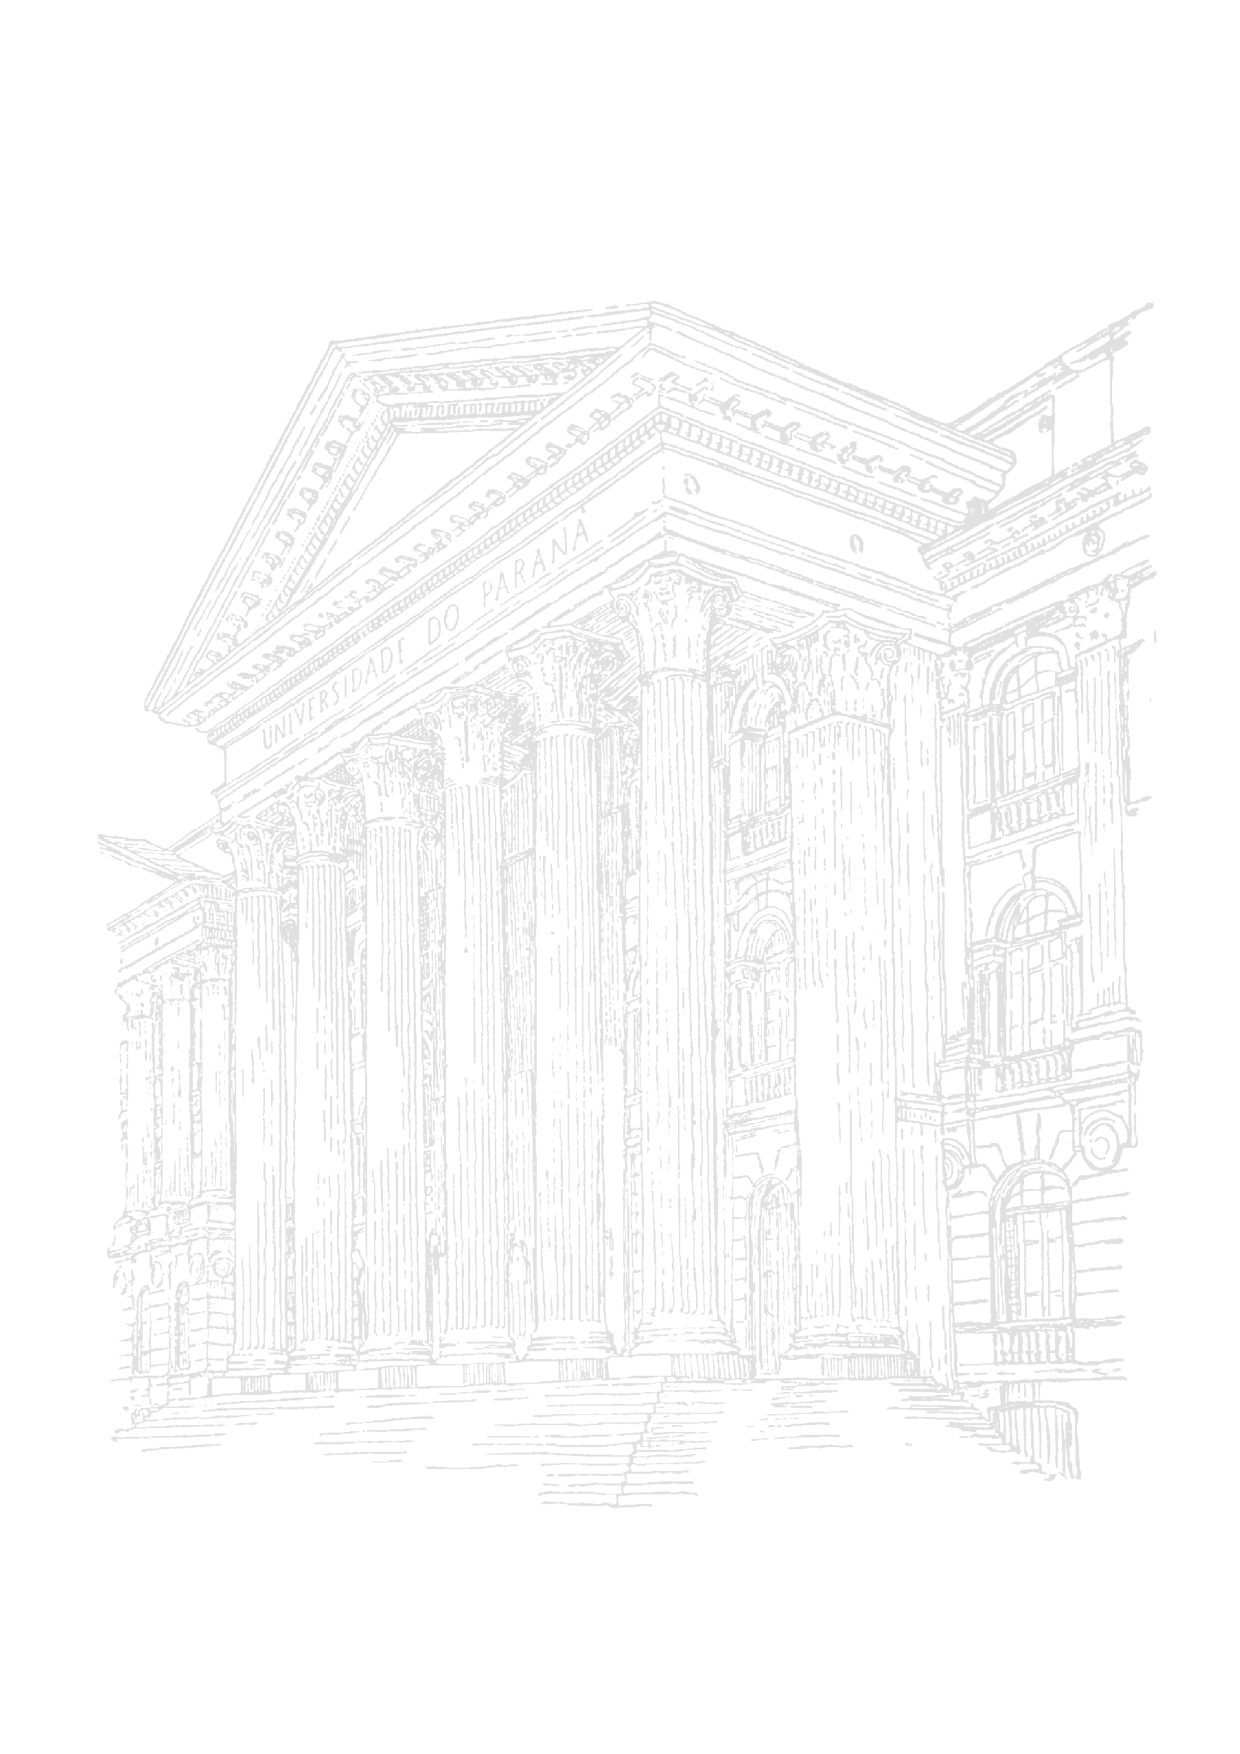
\includegraphics[width=\paperwidth,
  height=\paperheight]{Figuras/ufpr_bg}};
% ----------------------------------------------------------------------
\imprimircapa
% ----------------------------------------------------------------------
% folha de rosto
\imprimirfolhaderosto
% ----------------------------------------------------------------------

% \begin{dedicatoria}
%   \vspace*{\fill}
%   ...
%   \vspace*{\fill}
% \end{dedicatoria}
% ----------------------------------------------------------------------
% ficha catalográfica

% \begin{fichacatalografica}
%   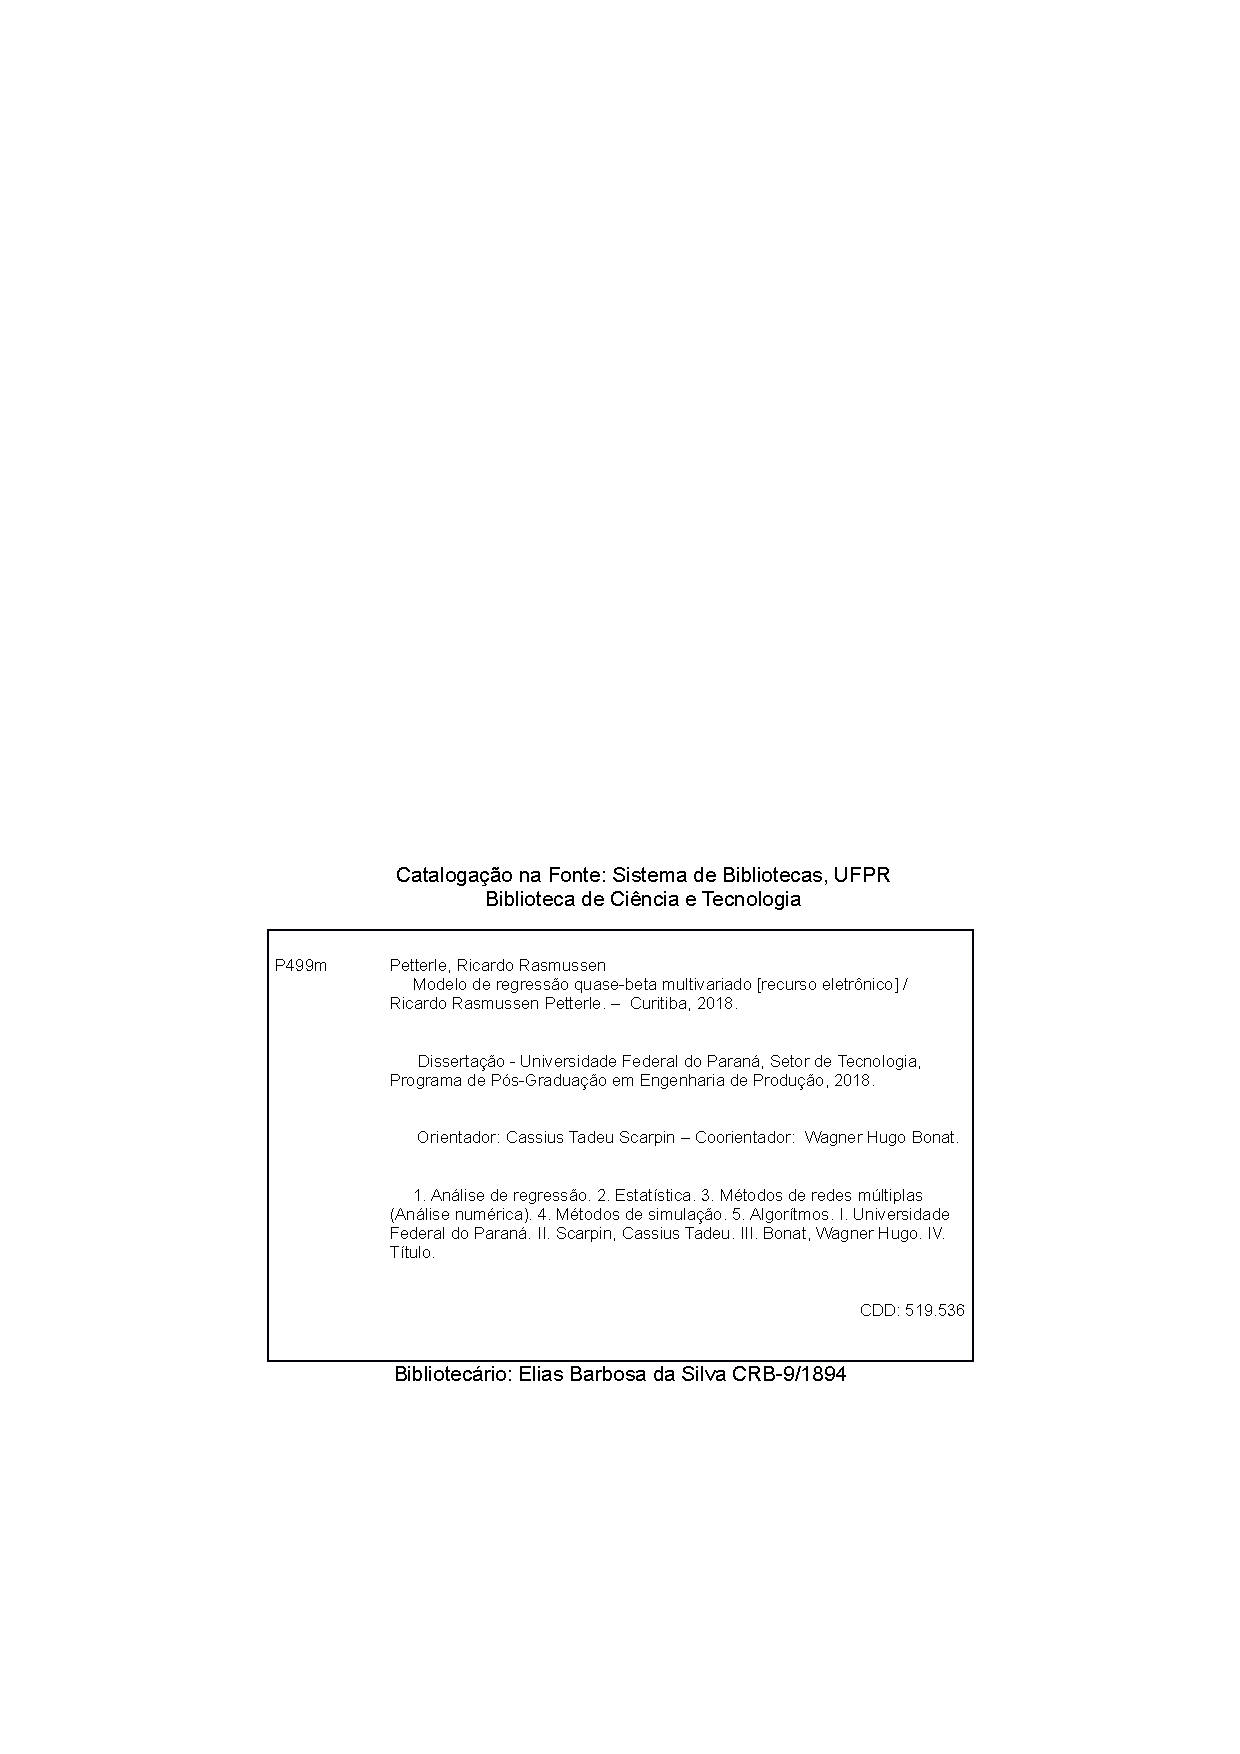
\includepdf{ficha.pdf}
% \end{fichacatalografica}
% ----------------------------------------------------------------------
% inserir folha de aprovação
% \begin{folhadeaprovacao}
%   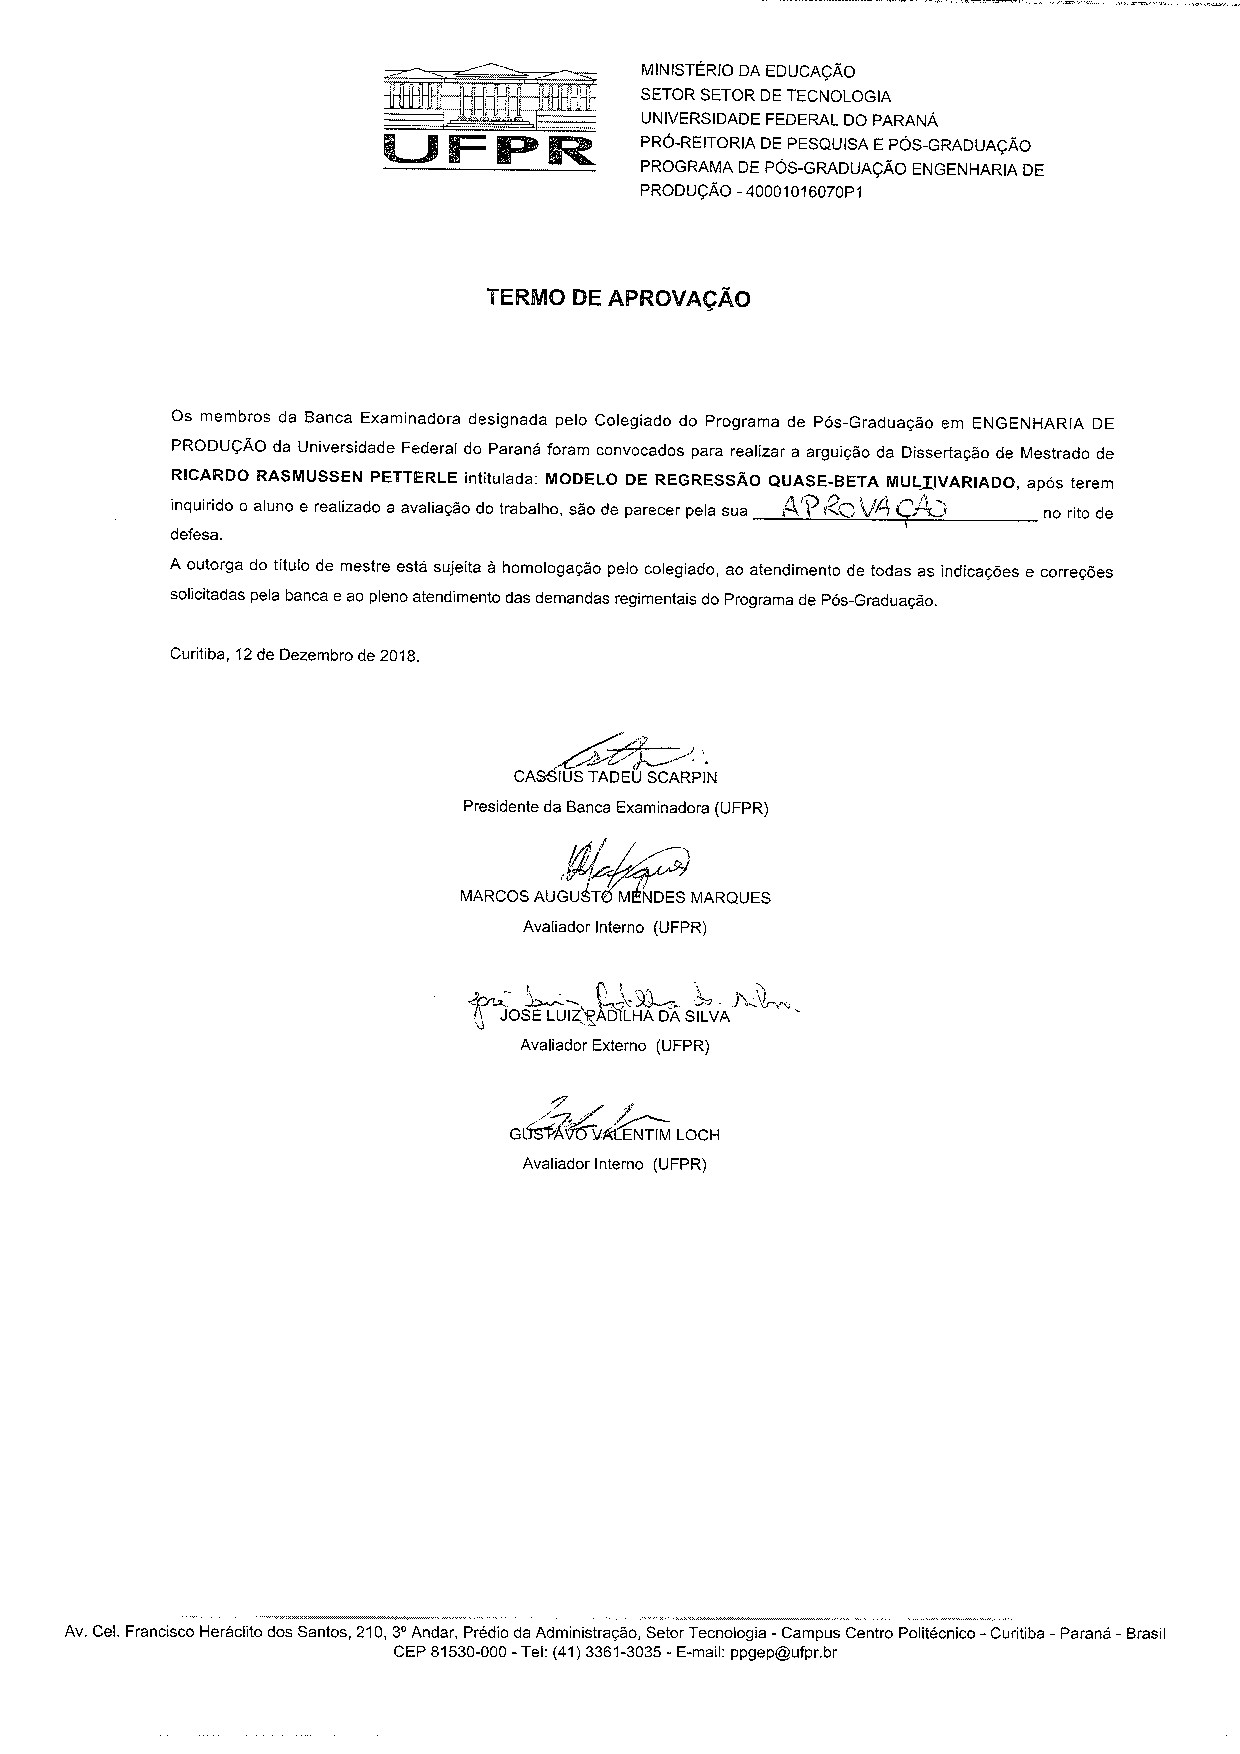
\includepdf{termo.pdf}
% \end{folhadeaprovacao}
\begin{folhadeaprovacao}
 \begin{center}
   {\ABNTEXchapterfont\large\imprimirautor}

   \vspace*{\fill}\vspace*{\fill}
   \begin{center}
     \ABNTEXchapterfont\bfseries\large\imprimirtitulo
   \end{center}
   \vspace*{\fill}

    \hspace{.45\textwidth}
    \begin{minipage}{.5\textwidth}
       \imprimirpreambulo
    \end{minipage}
   \vspace*{\fill}
 \end{center}

 Master thesis approved. XXX XX, 2020.

  \assinatura{\textbf{\imprimirorientador} \\ Supervisor}
  \assinatura{\textbf{Prof. PhD Paulo Justiniano Ribeiro Jr} \\
    Co-supervisor}
  \assinatura{\textbf{Prof. PhD ...} \\Internal Examinator - PPGMNE}
  \assinatura{\textbf{Prof. PhD ...} \\Internal Examinator - PPGMNE}
  \assinatura{\textbf{Prof. PhD ...} \\External Examiner - }

  \begin{center}
   \vspace*{0.5cm}
   {\large CURITIBA}
   \par
   {\large\imprimirdata}
   \vspace*{1cm}
 \end{center}

\end{folhadeaprovacao}
% ----------------------------------------------------------------------
\begin{dedicatoria}
  \vspace*{22.7cm}
  \begin{flushright}
    \begin{minipage}[H]{4.5cm}
      {To Celita and Olivio}
    \end{minipage}
  \end{flushright}
\end{dedicatoria}
% ----------------------------------------------------------------------
\begin{agradecimentos}
  ...
\end{agradecimentos}

\begin{epigrafe}
  \vspace*{\fill}
  \begin{flushright}
    \textit{"A simplicidade é o último grau de sofisticação".\\
      (Leonardo da Vinci)}
  \end{flushright}
\end{epigrafe}
% ----------------------------------------------------------------------
\newpage
\setlength{\absparsep}{18pt} % ajusta o espaçamento dos parágrafos do
                             % resumo
\setlength{\abstitleskip}{1cm} % adiciona mais um cm após o 'titulo' do
                               % resumo para ficar com 2cm
\begin{resumo}[]
  \vspace{-2cm}
  \begin{center}
    \bfseries{\large{\textsf{ABSTRACT}}}
  \end{center}
  \vspace{0.3cm}
  Failure time data
  \textbf{Keywords}: Competing risks.
\end{resumo}
% ----------------------------------------------------------------------
\newpage
\setlength{\absparsep}{18pt} % ajusta o espaçamento dos parágrafos do
                             % resumo
\setlength{\abstitleskip}{1cm} % adiciona mais um cm após o 'titulo' do
                               % resumo para ficar com 2cm
\begin{resumo}[]
  \begin{otherlanguage*}{brazil}
    \vspace{-2cm}
    \begin{center}
      \bfseries{\large{\textsf{RESUMO}}}
    \end{center}
    \vspace{0.3cm}
    Dados de tempos de falha
    \textbf{Palavras-chave}: Riscos competitivos.
  \end{otherlanguage*}
\end{resumo}
% ----------------------------------------------------------------------
\pdfbookmark[0]{\listfigurename}{lof}
\listoffigures*
\cleardoublepage
% ----------------------------------------------------------------------
\pdfbookmark[0]{\listtablename}{lot}
\listoftables*
\cleardoublepage
% ----------------------------------------------------------------------
% \begin{siglas}
% \item[Fig.] Area of the $i^{th}$ component
% \item[456] Isto éum número
% \item[123] Isto éoutro número
% \item[lauro cesar] este éo meu nome
% \end{siglas}
% ----------------------------------------------------------------------
\begin{simbolos}
\item[\(\mathbb{E}(\cdot)\)] The mathematical expectation of a random
  variable \(\cdot\)
\end{simbolos}
% ----------------------------------------------------------------------
\pdfbookmark[0]{\contentsname}{toc}
\tableofcontents*
\cleardoublepage
% ----------------------------------------------------------------------
\makepagestyle{abntheadings}
\makeevenhead{abntheadings}{\ABNTEXfontereduzida\thepage}{}{}
\makeoddhead{abntheadings}{}{}{\ABNTEXfontereduzida\thepage}
\makeheadrule{abntheadings}{\textwidth}{0in}
% ----------------------------------------------------------------------
\textual
% ----------------------------------------------------------------------
\chapter{Introduction}
\label{cap:intro}
Consider a cluster of random variables representing the time until the
occurrence of some event. These random variables are assumed to be
correlated, i.e. for some biological or environmental reason it is not
adequate to assume independence between them. Also, we may be interested
in the occurrence of not only one specific event, having in practice a
competition of events to see which one happens first, if it
happens. Such events may also be of low probability albeit severe
consequences, this is the moment when the cluster correlation makes its
difference: the occurrence of an event in a cluster member should affect
the probability of the same happening in the others.

A realistic context that fits perfectly with the framework described
above is the study of disease incidence in family members, where each
member is indexed by a random variable and each cluster consists of a
familiar structure. More specifically, we are interested in what is
called \textit{family studies}. Besides the dependence between family
members, this kind of data is characterized by being consisted of big
samples, or even a population, and having a lot of clusters/families of
small size. The inspiration to these kinds of problems came from the
work developed in \citeonline{SCHEIKE}, where they studied breast cancer
incidence in mothers and daughters but using a nontrivial estimation
framework. Based on that, the aim of this thesis is to propose a simpler
estimation framework taking advantage of several \textit{state-of-art}
computational libraries and see how far we can go in several
scenarios. Until now we have just contextualized, we still need to
introduce the methodology. To do this, some definitions and theoretical
contexts are welcome.

When the object under study is a random variable representing the time
until some event occurs, we are in the field of \textit{failure time
data} \cite{kalb&prentice}. The occurrence of an event is generally
denoted \textit{failure}, and major areas of application are biomedical
studies and industrial life testing. In this thesis, we maintain our
focus on the former. As common in science, same methodologies can
receive different names depending on the area. In industrial life
testing is performed what is called a \textit{reliability analysis}; in
biomedical studies is performed what is called
\textit{survival analysis}. Generally, the term \textit{survival} is
applied when we are interested in the occurrence of only one event, a
\textit{failure time process}. When we are interested in the occurrence
of more than one event we enter in the yard of \textit{competing risks}
and \textit{multistate} models. A visual aid is presented on
\autoref{fig:intro1} and a comprehensive reference is
\citeonline{kalb&prentice}.

Failure time and competing risks processes may be seen as particular
cases of a multistate model. Besides the number of events (states) of
interest, the main difference between a multistate model and its
particular cases is that only in the multistate scenario we may have
transient states, using a \textit{stochastic process} language. In the
particular cases, all states besides the initial state 0, are absorbents
- once you reached it you do not leave. The simplest multistate model
that exemplify this behavior is the illness-death model,
\autoref{fig:intro1}~C), where a patient (initially in state 0) can get
sick (state 1) or die (state 2); if sick it can recover (returns to
state 0) or die. We work in this thesis only with competing risks
processes, and for each patient we need the time (age) until the
occurrence, or not, of the event.

\begin{figure}[H]
 \setlength{\abovecaptionskip}{.0001pt}
 \caption{ILLUSTRATION OF MULTISTATE MODELS FOR A A) FAILURE TIME
          PROCESS; B) COMPETING RISKS PROCESS; AND C) ILNESS-DEATH
          MODEL, THE SIMPLEST MULTISTATE MODEL}
 \vspace{0.5cm}\centering
 \tikzfig{fig1}\\
 \vspace{0.5cm}
 \begin{footnotesize}
  SOURCE: The author~(2021).
 \end{footnotesize}
 \label{fig:intro1}
\end{figure}

When for some known or unknown reason we are not able to see the
occurrence of an event, we have what is denoted \textit{censorship}.
Still in the illness-death model, during the period of follow up the
patient may not get sick or die, staying at state 0. This is denoted
\textit{right-censorship}; if a patient is in state 1 at the end of the
study, we are \textit{censored} to see him reaching the state 2 or
returning to state 0. This is the inherent idea to censorship and must
be present in the modeling framework, thus arriving in the so-called
\textit{survival models} \cite{kalb&prentice}.

A survival model deals with the survival experience. Usually, the
survival experience is modeled in the \textit{hazard} (failure rate)
scale and it can be expressed for a subject \(i\) as
\begin{equation}
  \lambda(t \mid \bm{x}_{i}) =
  \lambda_{0}(t) \times c(\bm{x}_{i} \bm{\beta})
  \quad \text{at time}~t,
  \label{eq:intro1}
\end{equation}
i.e. as the product of an arbitrary baseline hazard function
\(\lambda_{0}(\cdot)\), with a specific function form \(c(\cdot)\), that
will depend on the probability distribution to be chosen for the failure
time and on predictors/covariates/explanatory/independent variables
\(\bm{x}_{i} = [x_{1}~\dots~x_{p}]\), where \(\bm{\beta}^{\top} =
[\beta_{1}~\dots~\beta_{p}]\) is the parameters vector.

This structure is specified for a failure time process, as in
\autoref{fig:intro1}~A). Nevertheless, the idea is easy to extend. We
basically have the \autoref{eq:intro1}'s model to each cause-specific
(in a competing risks process) or transition (in a multistate process).
For competing risks, the probable most famous approach is the
\citeonline{fine&gray} subdistribution model. A complete and extensive
detailing can be, again, found in \citeonline{kalb&prentice}.

In this work we approach the case of clustered competing risks. Besides
the cause-specific structure, we have to deal with the fact that the
events are happening in related individuals. This configures what is
denoted \textit{family studies}, i.e. we have a cluster/group/family
dependence that needs to be considered, accommodated, and modeled. This,
possible, dependence is something that we do not actually measure but
know (or just suppose) that exists. In the statistical modeling language
this characteristic receives the name of \textit{random} or
\textit{latent effect}.

A survival model with a latent effect, association, or unobserved
heterogeneity, is denoted \textit{frailty model}
\cite{frailty78,frailty79,liang95,petersen98}. In its simplest form, a
frailty is an unobserved random proportionality factor that modifies the
hazard function of an individual, or of related individuals. Frailty
models are extensions of \autoref{eq:intro1}'s model, and its use
implies challengeable likelihood functions (statistical objective
functions) and inference routines done via elaborated and slow
expectation–maximization (EM) algorithms \cite{nielsen92,klein92} or
inefficient Markov chain Monte Carlo (MCMC) schemes \cite{hougaard00}.
With multiple survival experiences, the general idea is the same but
with even more challengeable likelihoods
\cite{prentice78,larson85,kuk92,therneau00}.

In the competing risks setting, the hazard scale (focusing on the
cause-specific hazard) is not the only possible scale to work on. A more
attractive possibility is to work on the probability scale
\cite{andersen12}, focusing on the cause-specific cumulative incidence
function (CIF). Besides the within-family dependence, in family studies
there is often a strong interest in describing age at disease onset,
which is directly described by the cause-specific CIF. The CIF is the
cumulative probability of experiencing a failure by a given competing
cause along the time. Therefore, making the probability scale a more
attractive and logical choice. Since the CIF plays a central role in
this master thesis, it will be formally defined later in a place with
greater emphasis.

Besides the CIF specification itself, the known works with clustered
competing risks data in the probability scale, differ in terms of
likelihood construction and parameters estimation routines. There is a
lack of methodology predominance in the literature, but with its
majority being designed for bivariate CIFs, where increasing the CIF's
dimension is a limitation. Some of the existing options are
\begin{itemize}
 \item Nonparametric approaches \cite{cheng07,cheng09};
 \item Linear transformation models \cite{fine99,gerds12};
 \item Semiparametric approaches based on
  \begin{itemize}
   \item Composite likelihoods \cite{shih,SCHEIKE};
   \item Estimating equations \cite{cheng&fine12,crossoddsratioSCHEIKE};
   \item Copula models \cite{semiparametricSCHEIKE};
   \item Mixture models \cite{naskar05,shi13}.
  \end{itemize}
\end{itemize}

With the definitions and the theoretical context being made, let us be
more specific. To work with competing risks data on the probability
scale plus a latent structure allowing for within-cluster dependence of
both risk and timing, \citeonline{SCHEIKE} proposed a pairwise composite
likelihood approach based on the factorization of the cause-specific CIF
as the product of a cluster-specific risk level function with a
cluster-specific failure time trajectory function. A composite approach
\cite{lindsay88, cox&reid04, varin11} is a valid alternative to a full
likelihood analysis in high-dimensional situations when a full approach
is too computational costly or even inviable. A clear advantage of this
approach is that we do not need to care about a joint distribution
specification, which generally translates also into a computational
advantage. A disadvantage is the likelihood function specification,
which becomes much more challengeable, besides the number of small
details to workaround from the fact of being working with not an exact
likelihood function.

We do not have any guarantees that a full likelihood inference procedure
is not viable here, so we try to reach the same goal of
\citeonline{SCHEIKE} albeit with a simpler maximum likelihood estimation
framework taking advantage of \textit{state-of-art} software, something
still not so common in the statistical modeling community. This simpler
framework is based on a generalized linear mixed model (GLMM). Instead
of concentrating on failure time data and consequently having a
survival/frailty model based on the hazard scale, or using a composite
approach (or any other of the options listed above), we just build the
joint/full likelihood function (a multinomial model with its link
function based on the cluster-specific CIF, accouting for an appropriate
latent effects structure), marginalize (integrate out the latent
effects) and optimize it. A Fisherian approach per se.

In a standard linear model we assume that the response
variable \(Y_{i}\), conditioned on the covariates \(\bm{x}_{i}\),
follows a normal/Gaussian distribution and what we do is to model its
mean, \(\mu_{i} \equiv \mathbb{E}(Y_{i} \mid \bm{x}_{i})\), via a linear
combination. As much well explained in \citeonline{GLM72}, with the aid
of a \textit{link function} \(g(\cdot)\), this idea is generalized to
distributions of the \textit{exponential family}. Many of its members
are useful for practical modelling, such as the Poisson (for counting
data), binomial (dichotomic data), gamma (continuous but positive) and
Gaussian (continuous data) distributions. This extended framework
received the name of generalized linear models (GLMs) \cite{GLM72}, and
is probably the most popular statistical modelling framework. A
comprehensive reference is \citeonline{GLM89}.

 Despite its flexibility, the GLMs are not suitable for dependent
data. For the analysis of such data, \citeonline{laird82} proposed the
random effects regression models for longitudinal/repeated-measures data
analysis. \citeonline{breslow93} presented the GLMMs for the analysis of
non-Gaussian outcomes. What makes a GLM into a GLMM is the addition of a
latent effect \(\bm{u}\) (then, \textit{m}ixed) into the mean
structure. The mean structure of a standard GLMM for a subject \(i\) is
defined as
\[
  g(\mu_{i}) = \bm{x}_{i}\bm{\beta} + \bm{z}_{i}\bm{u},
  \quad \bm{u} \sim \text{Multivariate Normal}(\bm{0},\bm{\Sigma})
\]
where the latent effect is assumed to follow a multivariate Gaussian
distribution of zero mean and a parametrized variance-covariance matrix
\(\bm{\Sigma}\). Its correct linkage to the mean structure is made
through the \(i^\text{th}\) vector row of a design-matrix \(\bm{Z}\).
The covariates are into \(\bm{x}_{i}\), the \(i^\text{th}\) vector row
of a model-matrix \(\bm{X}\), with \(\bm{\beta}\) being a vector of
unknown parameters.

In the GLMM framework \cite{GLMM}, we can accommodate all competing
causes of failure and censorship with a multinomial probability
distribution, easily extend to any number of competing causes. The
within-cluster dependence is accommodated via the latent effect and the
cause-specific CIFs via the model's link function. The estimation and
inference are done via an efficient implementation and state-of-art
computational libraries provided through the R \cite{R21} package
TMB \cite{TMB}. The latent effects are handled out by means of an
efficient Laplace approximation \cite{corestats,patrao} and automatic
differentiation (AD)
\cite{corestats,peyre} routines.

\section{GOALS}

\subsection{General goals}

Propose and evaluate a maximum likelihood estimation approach of a
multinomial generalized linear mixed model (multiGLMM) to the cluster
and cause-specific cumulative incidence function (CIF) of clustered
competing risks data.

\subsection{Specific goals}

\begin{enumerate}
 \item Simulate from the model, i.e. generate synthetic data to study
       statistical properties.

 \item Write the model in the Template Model Builder (TMB) software,
       developed by \citeonline{TMB} and possibly the most efficient
       likelihood-based way of doing such task.

 \item Take advantage of TMB's functionalities with special attention to
       the computation of gradients and Hessians via a
       \textit{state-of-art} automatic differentiation (AD)
       implementation; and a joint likelihood marginalization via an
       efficient Laplace approximation routine.

 \item Assess the maximum likelihood estimation method embedded on TMB.
       Check its properties in our model for different complexity level
       in terms of parametric space and latent effect structures.

 \item Make exact likelihood-based inference to the cluster and
       cause-specific CIF of clustered competing risks data.
\end{enumerate}

\section{JUSTIFICATION}

In the biomedical statistical modeling literature, the study of disease
occurrence in related individuals receives the name of family studies.
Key points of interest are the within-family dependence and determining
the role of different risk factors. The within-family dependence may
reflect both disease heritability and the impact of shared environmental
effects. The role of different risk factors arrives in the class of
multivariate models, which options are limited in the statistical
literature. Thus, the number of statistical models for competing risks
data that accommodate the within-cluster/family dependence is even more
limited. Some modeling options are briefly commented in
\citeonline{SCHEIKE}, with his pairwise composite approach being
proposed as a new and better option to model the cause-specific
cumulative incidence function (CIF), describing age at disease onset, of
clustered competing risks data on the probability scale. We propose to
model the cause-specific CIF and accommodate the within-family
dependence in the same fashion (via a latent structure that allows the
absolute risk and the failure time distribution to vary between
families) but with an easier estimation framework, based on a
full-likelihood approach of a multinomial generalized linear mixed
model.

\section{LIMITATION}

This work restraint to the proposition and maximum likelihood estimation
method evaluation of a multinomial model for the cause-specific
cumulative incidence function (CIF) of competing risks data in the
context of family studies, with a latent effect structure to accommodate
within-family dependence with regard to both risk and timing. Family
studies are characterized by a considerable amount of clusters
(families) but with each one having a small number of elements. Given
its considerable model complexity, hypothesis tests; residual analysis;
and good-of-fit measures are not contemplated.

\section{THESIS ORGANIZATION}

This master thesis contains 6 chapters including this introduction.
\autoref{cap:methods} presents a systematic review of the main aspects
involved in the formulation, optimization, and implementation of a
generalized linear mixed model (GLMM). Given the modeling framework
overview, \autoref{cap:model} presents our multinomial GLMM (multiGLMM)
to model the cause-specific cumulative incidence function (CIF) of
clustered competing risks data. In \autoref{cap:datasets} we describe
the simulation procedure to generate synthetic data and present some
model particularities. In \autoref{cap:results} the obtained results are
presented, and in \autoref{cap:finalc} we discuss the contributions of
this thesis and present some suggestions for future work.

% END ==================================================================

% ----------------------------------------------------------------------
\chapter{Conjuntos de dados}
\label{cap:aplicacoes}
% ======================================================================

Este Capítulo descreve os dois conjuntos de dados que serão usados como
exemplos de aplicação no novo modelo de regressão, proposto no
\autoref{cap:multivariatemodel}. O primeiro conjunto se refere ao índice
de qualidade da água de reservatórios de usinas hidrelétricas operadas
pela COPEL no Estado do Paraná. Já o segundo conjunto de dados
corresponde ao percentual de gordura corporal de indivíduos avaliados no
Hospital de Clínicas da Universidade Federal do Paraná.

\section{CONJUNTO DE DADOS I: ÍNDICE DE QUALIDADE DA ÁGUA}
\label{cap:IQA}

\begin{table}[H]
  \centering
  \setlength{\abovecaptionskip}{.0001pt}
  \caption{ANÁLISE DESCRITIVA PARA O IQA POR TRIMESTRE E LOCAL}
  \label{tab:descIQA}
  \begin{tabular}{cccc}
    \hline
    \multirow{2}{*}{Trimestre} & \multicolumn{3}{c}{Local} \\
    \cline{2-4}  & Montante & Reservatório & Jusante \\
    \cline{2-4} 1   & $0,75\pm 0,11$   &  $0,80\pm 0,10$  &  $0,78\pm 0,10$  \\
    2  &  $0,79\pm 0,10$  &  $0,83\pm 0,06$   &  $0,83\pm 0,07$     \\
    3   &  $0,81\pm 0,07$   & $0,85\pm 0,05$   &  $0,83\pm 0,06$    \\
    4   & $0,76\pm 0,10$    &  $0,81\pm 0,08$    &  $0,79\pm 0,09$    \\
    \hline
  \end{tabular}
  \begin{footnotesize}
    \vspace{0.05cm}
    FONTE: O autor~(2018). \hspace{6.2cm}
    \vspace{-0.15cm}
  \end{footnotesize}
\end{table}

\vspace{-0.2cm}

\begin{figure}[H]
  \vspace{0.35cm}
  \setlength{\abovecaptionskip}{.0001pt}
  \caption{HISTOGRAMA~(A) E BOXPLOTS PARA O ÍNDICE DE QUALIDADE DA ÁGUA
    (IQA) POR TRIMESTRE~(B), LOCAL~(C) E USINAS~(D)}
  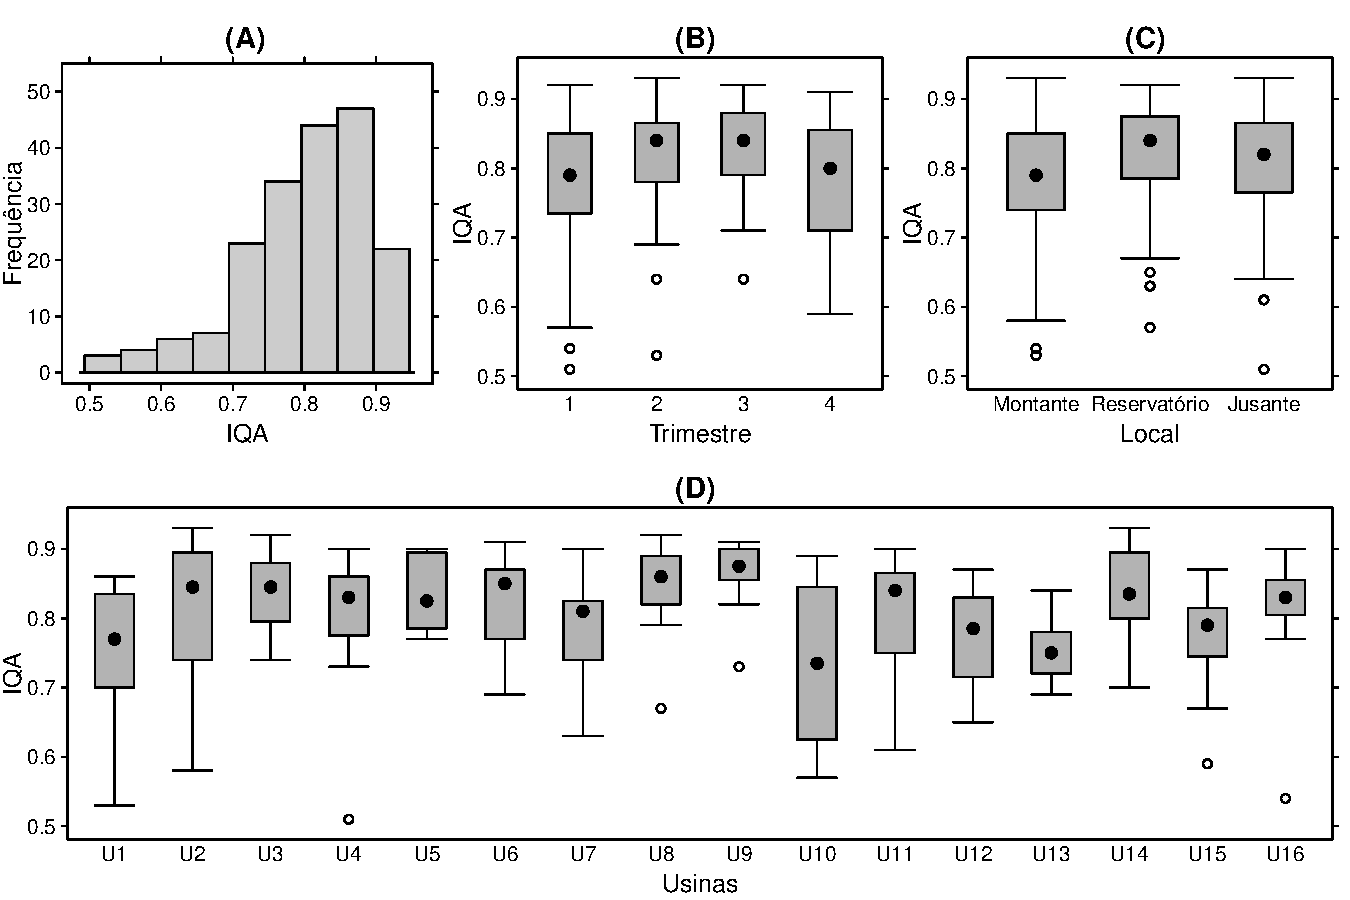
\includegraphics[width=0.95\textwidth]{Figure2.pdf}
  \begin{footnotesize}
    \vspace{-0.20cm}
    \centering
    FONTE: O autor~(2018).
    \vspace{0.15cm}
  \end{footnotesize}
  \label{fig:iqa1}
\end{figure}

Por fim, os resultados apresentados na~\autoref{fig:iqa1}~(D) mostram
que o IQA não é homogêneo entre as usinas, com um destaque maior para as
usinas 1, 2 e 10. É importante ressaltar que os resultados apresentados
na~\autoref{tab:descIQA} e~\autoref{fig:iqa1} se referem apenas a
análise descritiva e exploratória dos dados, onde são criadas hipóteses
que serão confirmadas somente após ajuste do modelo de regressão
proposto no~\autoref{cap:multivariatemodel}. No~\autoref{cap:apendiceA}
são apresentados gráficos boxplots para o IQA separado por trimestre e
local em função das usinas.

% ======================================================================
% ----------------------------------------------------------------------
\chapter{Fundamentação teórica}
\label{cap:fundamentacaoteorica}
% ======================================================================

Este Capítulo apresenta a fundamentação teórica que será usada nesta
dissertação. A~\autoref{cap:refteorico} apresenta um breve resumo dos
principais trabalhos relacionados ao assunto. A distribuição de
probabilidade beta e suas propriedades encontram-se
na~\autoref{cap:densbeta}. A~\autoref{cap:norta} apresenta o algoritmo
NORTA, que será usado para simular variáveis aleatórias beta
correlacionadas. A~\autoref{cap:betamodel} introduz o modelo de
regressão beta (univariado). Por fim, a~\autoref{cap:gof} apresenta
brevemente as medidas de bondade de ajuste usadas na comparação entre os
modelos.

\section{REVISÃO DA LITERATURA}
\label{cap:refteorico}

\section{DISTRIBUIÇÃO DE PROBABILIDADE BETA}
\label{cap:densbeta}

\begin{figure}[!htb]
  \centering
  \vspace{0.35cm}
  \setlength{\abovecaptionskip}{.0001pt}
  \caption{FUNÇÃO DE DISTRIBUIÇÃO BETA PARA DIFERENTES VALORES DE $\mu$
    COMBINADOS COM $\phi = (0,00001;~0,666;~4;~9;~23,99)$}
  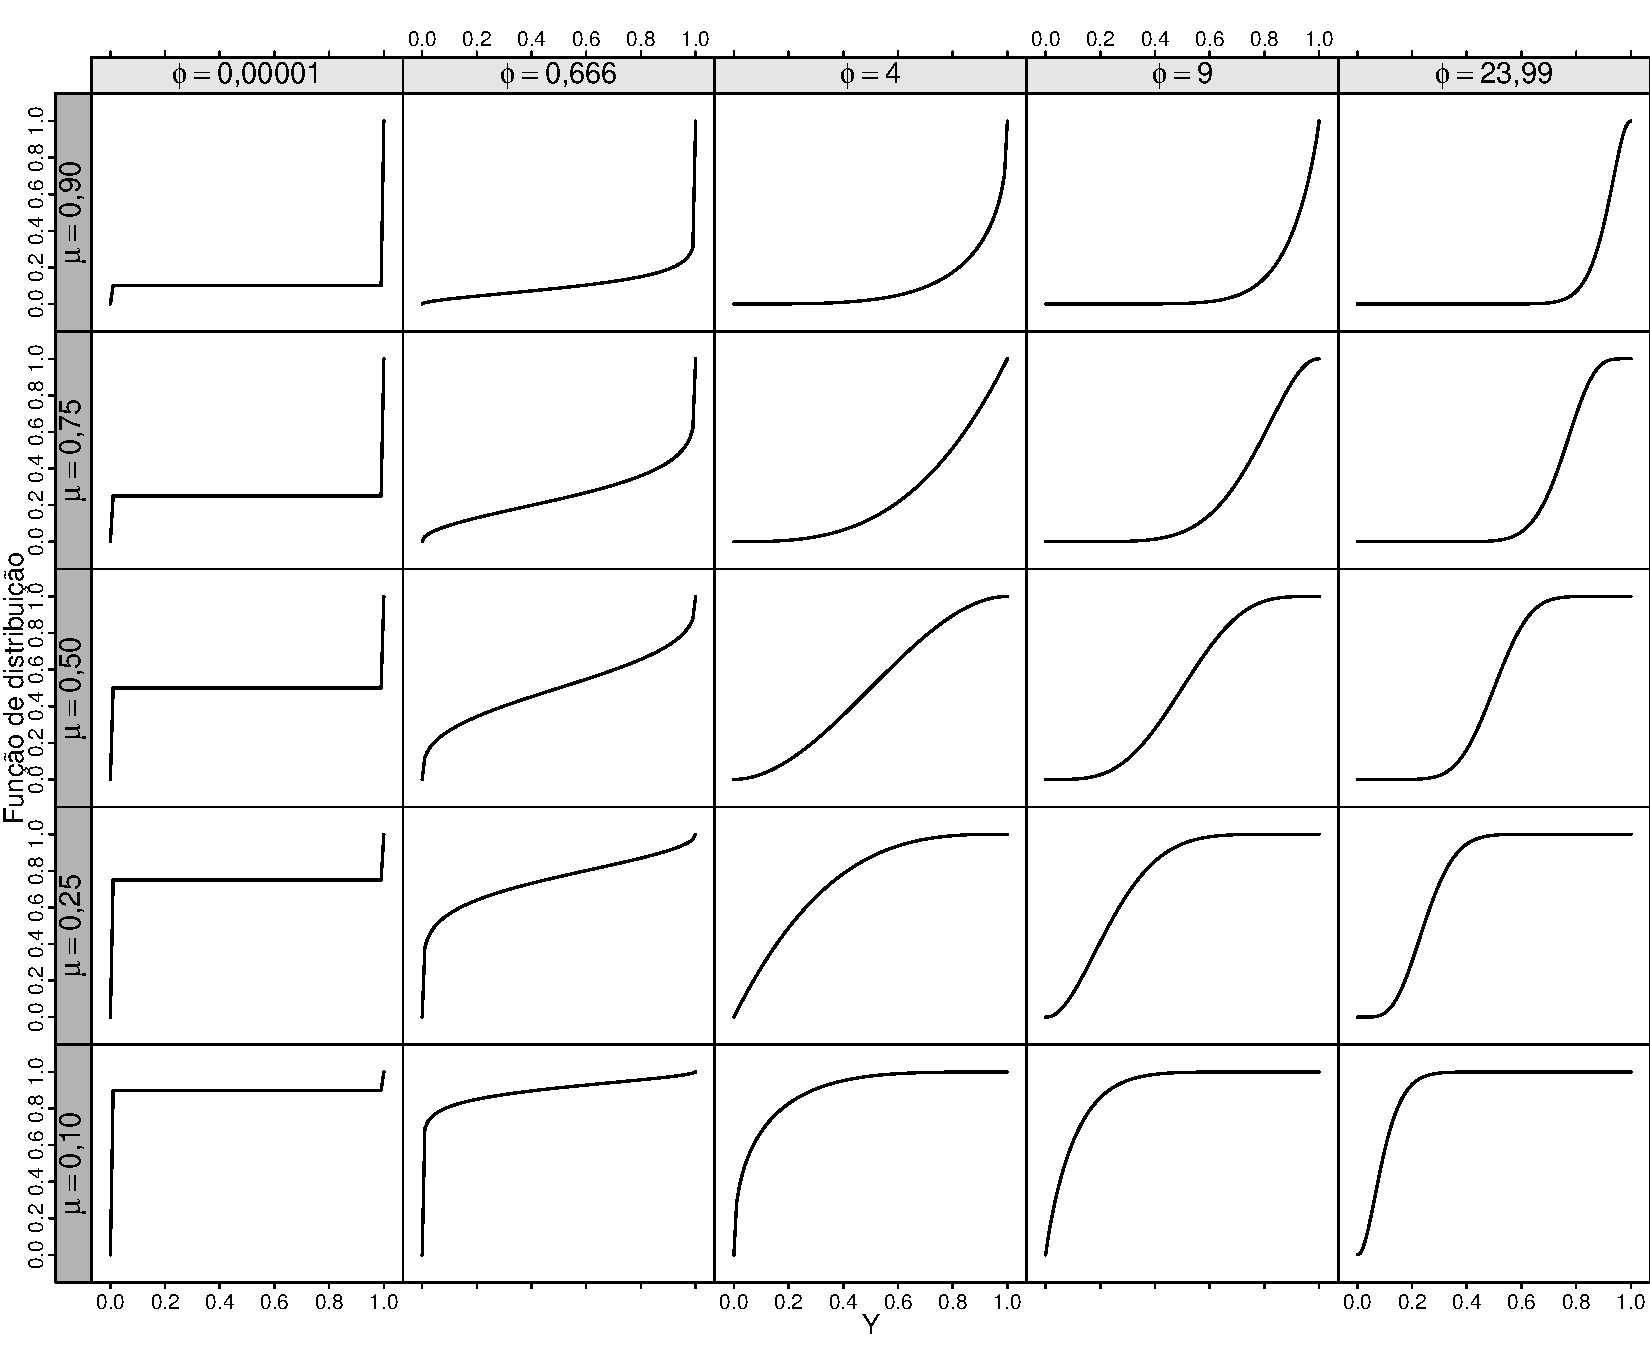
\includegraphics[width=.9\textwidth]{Figure6.pdf}
  \begin{footnotesize}
    \vspace{-0.1cm}
    FONTE: O autor~(2018).
    \vspace{0.15cm}
  \end{footnotesize}
  \label{fig:dbeta}
\end{figure}

\begin{figure}[H]
  \vspace{0.35cm}
  \setlength{\abovecaptionskip}{.00001pt}
  \caption{CÓDIGOS EM LINGUAGEM R PARA GERAÇÃO DE VARIÁVEIS ALEATÓRIAS
    BETA CORRELACIONADAS}
  \vspace{-0.5cm}
  \begin{program}[H]
    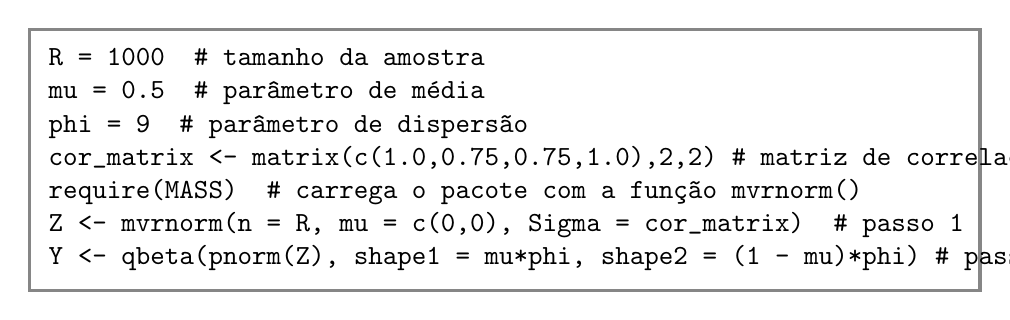
\begin{tikzpicture}
      \node [mybox] (box){
        \begin{minipage}{0.955\textwidth}
\begin{verbatim}
R = 1000  # tamanho da amostra
mu = 0.5  # parâmetro de média
phi = 9  # parâmetro de dispersão
cor_matrix <- matrix(c(1.0,0.75,0.75,1.0),2,2) # matriz de correlação
require(MASS)  # carrega o pacote com a função mvrnorm()
Z <- mvrnorm(n = R, mu = c(0,0), Sigma = cor_matrix)  # passo 1
Y <- qbeta(pnorm(Z), shape1 = mu*phi, shape2 = (1 - mu)*phi) # passo 2
\end{verbatim}
        \end{minipage}
      };
    \end{tikzpicture}
  \end{program}
  \vspace{-0.5cm}
  \begin{footnotesize}
    \centering
    FONTE: O autor~(2018).
    \vspace{-0.28cm}
  \end{footnotesize}
  \label{fig:steps1e2}
\end{figure}

% ======================================================================
% ----------------------------------------------------------------------
\chapter{Modelo de regressão multivariado}
\label{cap:multivariatemodel}
% ======================================================================

Este Capítulo apresenta o novo modelo de regressão usado para análise de
variáveis respostas limitadas multivariada, o qual será chamado por
modelo de regressão quase-beta multivariado. A~\autoref{cap:modelo}
apresenta a estrutura do modelo, enquanto a~\autoref{cap:estimacao}
apresenta o método proposto para estimação dos parâmetros de regressão e
dispersão. Por fim, a~\autoref{cap:diagnostics} adapta técnicas de
diagnóstico para o modelo proposto.

\section{MODELO DE REGRESSÃO QUASE-BETA MULTIVARIADO}
\label{cap:modelo}

% END ==================================================================
% ----------------------------------------------------------------------
\chapter{Resultados}
\label{cap:resultados}
% Neste Capítulo são apresentados os resultados de três estudos de
% simulação, além da análise dos dados apresentados no
% \autoref{cap:aplicacoes}. O primeiro estudo de simulação foi conduzido
% para investigar o comportamento do algoritmo NORTA (NOR\textit{mal To
%   Anything}) na simulação de variáveis aleatórias beta correlacionadas
% (\autoref{cap:simul1}). O segundo visou checar propriedades dos
% estimadores para os parâmetros de dispersão, no contexto de análise de
% dados longitudinais (\autoref{cap:simulLong}). E o terceiro foi
% delineado para explorar a flexibilidade dos estimadores para lidar com
% múltiplas respostas correlacionadas (\autoref{cap:simul2}). Por fim, a
% \autoref{cap:resultIQA} apresenta os resultados da análise dos dados
% referente ao índice de qualidade da água (IQA), enquanto a
% \autoref{cap:resultcorporal} apresenta os resultados correpondentes ao
% percentual de gordura corporal.

% \section{ESTUDOS DE SIMULAÇÃO}

% \subsection{Comportamento do algoritmo NORTA}
% \label{cap:simul1}

% \begin{figure}[H]
%   \vspace{0.4cm}
%   \caption{VALORES MÍNIMOS E MÁXIMOS PARA A CORRELAÇÃO ENTRE DUAS
%     VARIÁVEIS ALEATÓRIAS BETA EM FUNÇÃO DAS MÉDIAS MARGINAIS E
%     DIFERENTES VALORES DO PARÂMETRO $\phi$}
%   \setlength{\abovecaptionskip}{.0001pt}
%   \vspace{-0.38cm}
%   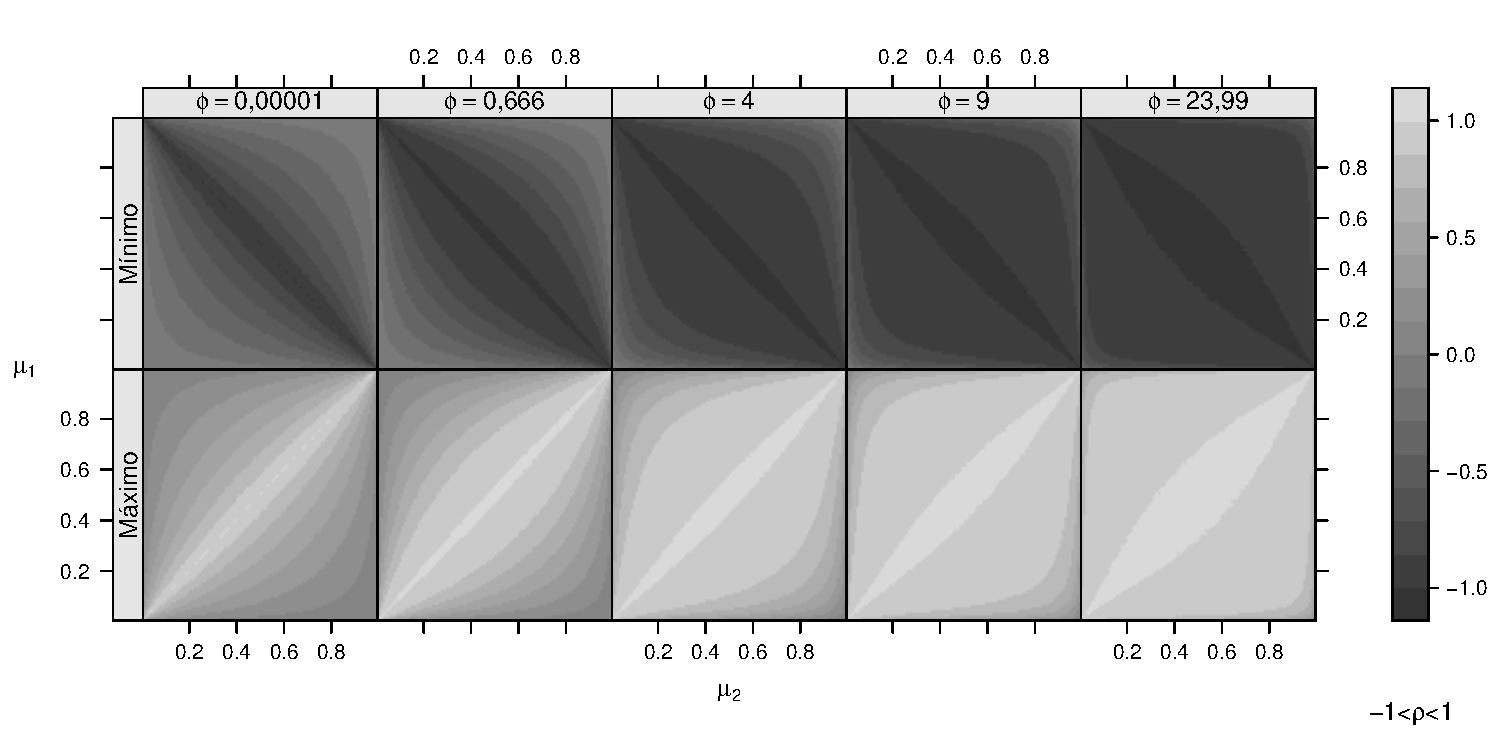
\includegraphics[width=16.0cm,height=7.6cm]{Figure10.pdf}
%   \vspace{-0.7cm}
%   \begin{footnotesize}
%     \centering
%     FONTE: O autor~(2018).
%     \vspace{0.15cm}
%   \end{footnotesize}
%   \label{fig:simulnorta}
% \end{figure}

% \begin{equation}
%   \label{eq:linearPredIQA}
%   g(\mu_{jki}) = \beta_0  + \beta_{1j}~\texttt{local}_{ji} + \beta_{2k}~\texttt{trimestre}_{ki},
% \end{equation}
% \noindent
% Na sequência, ajustou-se o modelo de regressão quase-beta multivariado
% aos dados do IQA, considerando as quatro estruturas acima mencionadas
% além de especificar a função de ligação \textit{logit} para o preditor
% linear~(\autoref{eq:linearPredIQA}).

% END ==================================================================
% ----------------------------------------------------------------------
\chapter{Considerações finais}
\label{cap:considefinais}
% O objetivo geral desta dissertação foi propor um novo modelo de
% regressão para análise de variáveis respostas limitadas multivariada. O
% modelo foi especificado usando apenas suposições de primeiro e segundo
% momentos. Para estimação dos parâmetros, adotou-se uma abordagem que
% combina as funções de estimação quase-score e Pearson para estimação dos
% parâmetros de regressão e dispersão, respectivamente. Assim, o modelo
% proposto nesta dissertação segue o estilo de quase-verossimilhança
% apresentado, onde a especificação do modelo é feita pela combinação da
% função de variância da distribuição binomial com as tradicionais funções
% de ligação para dados binários.

\section{FUTURE WORKS}

% END ==================================================================
% ----------------------------------------------------------------------
\setlength{\afterchapskip}{\baselineskip}
% ----------------------------------------------------------------------
\bibliography{references}
% ----------------------------------------------------------------------
\postextual
% ----------------------------------------------------------------------
% \begin{apendicesenv}
% \partapendices
% \addcontentsline{toc}{chapter}{\hspace{2.105cm}APPENDIX}
% \renewcommand{\ABNTEXchapterfontsize}{\ABNTEXsectionfont}
% \end{apendicesenv}
% ----------------------------------------------------------------------
% \begin{anexosenv}
% \partanexos
% \addcontentsline{toc}{chapter}{\hspace{2.105cm}ANNEX}
% \renewcommand{\ABNTEXchapterfontsize}{\ABNTEXsectionfont}
% \end{anexosenv}
%-----------------------------------------------------------------------
\phantompart
\printindex
%-----------------------------------------------------------------------
\end{document}
% END ==================================================================